\documentclass{beamer}
\usepackage{amsmath}
\usepackage{graphicx}
\usepackage{url}
\usepackage{fancyvrb}
\usepackage{color}
\usepackage{tikz}
%\usepackage{movie15}
\usepackage{multimedia}
\usepackage{hyperref}

\usetikzlibrary{shapes,arrows}

% This is the file main.tex
\mode<presentation>
{
  \usetheme{Warsaw}
  % or ...

  \setbeamercovered{transparent}
  % or whatever (possibly just delete it)
}
\usepackage[english]{babel}
% or whatever

\usepackage[latin1]{inputenc}
% or whatever

\usepackage{times}
\usepackage[T1]{fontenc}
\title[Efforts on OPAL towards Dark current \& Multipacting Simulation]{Status of OPAL Boundary Geometry Feature and Surface Emission Models for Dark current and Multipacting Simulation
 }
\author[Chuan Wang]{Chuan Wang \\
AMAS Group, PSI \& China Institute of Atomic Energy \\
chuan.wang@psi.ch; cwang@ciae.ac.cn}
\date{\today}
\AtBeginSubsection[]
{
  \begin{frame}<beamer>{Outline}
    \tableofcontents[currentsection,currentsubsection]
  \end{frame}
}

\begin{document}
\begin{frame}
\titlepage
\end{frame}
%\begin{frame}{Outline}
%  \tableofcontents
  % You might wish to add the option [pausesections]
%\end{frame}
\section*{Outlines}
\begin{frame}
\tableofcontents
\end{frame}
\begin{frame}
\frametitle{THE GOAL OF THE WORK}
\begin{itemize}
\item Extend OPAL to handle the complex boundary.

\item Provide field emission model and a reduced model of randomly generated electrons for dark current study (CTF3 gun, new gun...)

\item Provide feasible multipacting model primarily for cyclotrons, including models of field emission, secondary emission...
\end{itemize}
\end{frame}
\section{New geometry feature: particle-boundary collision test model}
\subsection{Basic idea: line segment-triangle intersection (LSTI) test}
\begin{frame}
\frametitle{LINE SEGMENT-TRIANGLE INTERSECTION TEST}
\begin{columns}
\begin{column}[t]{5.5cm}
\begin{figure}[H]
\begin{center}

\scalebox{0.7}{
\begin{tikzpicture}
\usetikzlibrary{arrows}
\draw [->,black,-latex] (-1.5,0) -- (1.5,0);
\draw [->,black,-latex] (-1.5,0) -- (-1.5,2);
\draw (1.5,0) -- (0.0,2);
\draw  [<-,black,latex-](0.0,2) -- (-1.5,0.0);
\draw [->,black,-latex,dashed] (-1.5,0) -- (0.5,0.5);
\node[below] (w) at (-0.15,0.5) {$\vec{w}$};
\draw[dashed] (0.5,0.5) -- (-1.18,0.5);
\draw[dashed] (0.5,0.5) -- (0.01,0.0);
\node[above] (ti) at (-1.18,0.5) {$t_i$};
\node[below] (si) at (0.01,0.0) {$s_i$};
\node[above] (t0) at (-1.7,0.) {$\mathbf{t_0}$};
\node[right] (t1) at (1.5,0) {$\mathbf{t_1}$};
\node[above] (t2) at (0.0,2.0) {$\mathbf{t_2}$};
\node[above] (n) at (-1.5,2) {$\vec{n}$};
\node[above] (v) at (-0.5,1.5) {$\vec{v}$};
\node[below] (u) at (1.2,0.0) {$\vec{u}$};
\path[draw=black,fill=black] (0.0,2.0) circle (2pt);
\path[draw=black,fill=black] (1.5,0.0) circle (2pt);
\path[draw=black,fill=black] (-1.5,0.0) circle (2pt);
\draw (-3.5,-1) -- (2.5,-1);
\draw (2.5,-1) -- (5,3);
\draw (0,3) -- (5,3);
\draw (-3.5,-1) -- (0,3);
\draw (0.5,0.5) -- (1.6,5);
\path[draw=black] (0.5,0.5) circle (2pt);
\node[above] (I) at (0.5,0.5) {$\mathbf{I}$};
\node[right] (x0) at (1.6,5) {$\mathbf{x_0}$};
\draw[dashed] (0.5,0.5) -- (-0.1,-1.9);
\node[right] (x1) at (0.0,-1.9) {$\mathbf{x_1}$};
\node[right] (ri) at (1,2.5) {$r_i$};
\path[draw=black,fill=black] (-0.1,-1.9) circle (2pt);
\path[draw=black,fill=black] (1.6,5) circle (2pt);
\end{tikzpicture}
}
\end{center}
%\caption{Line segment-triangle intersection()\label{fig:L-T}}
\end{figure}
\pause
\end{column}
\begin{column}[t]{5cm}
\begin{itemize}

\item  $\mathbf{x}_0,\mathbf{x}_1$ are position of a particle.

\pause

\item Triangle $\mathbf{t}_0,\mathbf{t}_1,\mathbf{t}_2$ is one piece of triangulated boundary surface.

\pause

\item Using D.Sunday's\cite{LT} Line-Triangle intersect algorithm.
\pause
\item Precomputed triangle normal.
\end{itemize}
\end{column}
\end{columns}
\end{frame}
\subsection{Early rejection strategy}
\begin{frame}
\frametitle{MOTIVATION}
\begin{itemize}

\item LSTI test is accurate but time consuming. 
\pause
\item Solution: early rejection strategy.
\end{itemize}
\end{frame}
\begin{frame}
\frametitle{EARLY REJECTION}
\begin{columns}
\begin{column}[t]{5.5cm}
\begin{figure}[H]
\begin{center}

/Users/adelmann/svnwork/adelmann/papers/figures/Latex-Figures/2d_grid.tikz
\end{center}
%\caption{Line segment-triangle intersection()\label{fig:L-T}}
\end{figure}
\pause
\end{column}
\begin{column}[t]{5cm}
\begin{itemize}

\item Use uniformed boxes to facilitate the particle searching.
\pause
\item Shield like boundary box .
\pause
\item Direction of momentum and triangle normal are also evaluated.

\end{itemize}
\end{column}
\end{columns}
\end{frame}

\section{Surface emission physics models}
\subsection{Field emission model}
\begin{frame}
\frametitle{ELECTRON QUANTUM TUNNELING AT HIGH FIELD}
\begin{itemize}
\item Fowler-Nordheim formula induced by \cite{FN} and implemented for dark current simulation by \cite{DE}: $J(\mathbf{r},t) = \frac{A(\beta E)^2}{\varphi t(y)^2}\exp{(\frac{-B v(y)\varphi^{3/2}}{\beta E})}$
\pause
\item $J(\mathbf{r},t)$: current density in position $\mathbf{r}$ and time $t$; $\varphi$: work function; $\beta$: field enhancement factor; $E$: electric field in the normal direction of surface; $A$ and $B$ are empirical constants;  
\pause
\item Functions $v(y)$ and $t(y)$ represents the image charge effects, detailed in \cite{BC} with: $y = \sqrt{\frac{e^3}{4\pi\varepsilon}}\frac{\sqrt{\beta E}}{\varphi} = 3.795\times10^{-5}\frac{\sqrt{\beta E}}{\varphi}$.
\end{itemize}
\end{frame}
\begin{frame}
\frametitle{SPACE CHARGE CONSIDERATION}
\begin{itemize}
\item Child-Langmuir law
\pause
\begin{align*}
J(\mathbf{r},t) & =\frac{4\varepsilon_0}{9}\sqrt{2\frac{e}{m}}(\frac{V^{3/2}}{d^2})\\
 & =\frac{4\varepsilon_0}{9}\sqrt{2\frac{e}{m}}(\frac{E^{3/2}}{d^{1/2}})
\end{align*}
\pause
\item A multi-grid space charge solver developed by \cite{SV} is already implemented in OPAL. But the ability to handle the complex boundary is not available yet.

\end{itemize}
\end{frame}
\subsection{Secondary emission model}
\begin{frame}
\frametitle{SECONDARY EMISSION MODEL}
\begin{columns}
\begin{column}[t]{6.5cm}
\begin{figure}[H]
\begin{center}

\scalebox{0.7} {
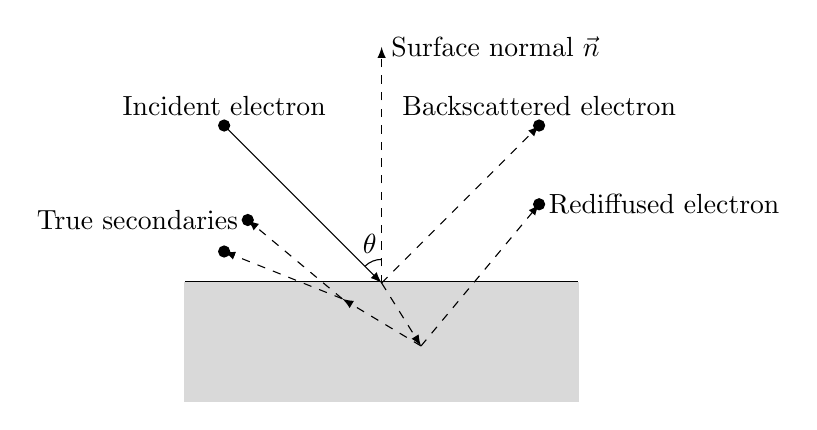
\begin{tikzpicture}
\usetikzlibrary{arrows}
\draw [very thick] (-2.5,0) -- (2.5,0);
\draw[gray!30,fill=gray!30] (-2.5,-1.5) rectangle (2.5,0); 
\draw [->,dashed,-latex] (0,0) -- (0,3);
%\node[below] (w) at (-0.15,0.5) {$\vec{w}$};
\node[right] (n) at (0,3) {Surface normal $\vec{n}$};
\path[draw=black,fill=black] (-2,2.0) circle (2pt);
\node[above] (electron) at (-2,2) {Incident electron};
\path[draw=black,fill=black] (2,2.0) circle (2pt);
\node[above] (electron1) at (2,2) {Backscattered electron};
\draw [->,-latex] (-2,2.0) -- (0,0);
\draw [dashed,->,-latex]  (0,0) -- (2,2.0);
\draw [dashed,->,-latex]  (0,0) -- (0.5,-0.8);
\draw [dashed,->,-latex]  (0.5,-0.8) -- (2,1);
\path[draw=black,fill=black] (2,1.0) circle (2pt);
\node[right] (electron1) at (2,1) {Rediffused electron};
\draw [dashed,->,-latex]  (0.5,-0.8) -- (-0.5,-0.2);
\draw [dashed,->,-latex] (-0.5,-0.2) -- (-2,0.4);
\draw [dashed,->,-latex] (-0.5,-0.2) -- (-1.7,0.8);
\path[draw=black,fill=black] (-2,0.4) circle (2pt);
\path[draw=black,fill=black] (-1.7,0.8) circle (2pt);
\node[left] (electron1) at (-1.7,0.8) {True secondaries};
\node[above] (theta) at (-0.15,0.25) {$\theta$};
\draw (0,0.3) arc (90:135:0.3);
\end{tikzpicture}
}
\end{center}
%\caption{Line segment-triangle intersection()\label{fig:L-T}}
\end{figure}

A Probabilistic model developed by \cite{SE}
\end{column}
\pause
\begin{column}[t]{5cm}
\begin{itemize}
\item Mathematically self-consistent
\pause
\item Phenomenological- don't involve secondary physics but fit the data.
\pause

\item A serial of parameters to fit the measured SEY data.
\pause
\item The Monte Carlo technique has been used

\end{itemize}
\end{column}
\end{columns}
\end{frame}
\section{Current results}
\subsection{Dark current simulation with field emission model}
\begin{frame}
%\begin{center}
%\begin{figure}[ht]
%\includemovie[
%  poster, % shows initial frame before play begins
%  controls,    % controls are only available on a Mac (they will not appear on windows.) 
  % (if no controls are used, then you can double click the movie to start it.)
%  repeat, % repeat the movie over and over.
% text=(Loading movie...)  % text shown while loading movie
%]{6cm}{6cm}{alivetest.avi}
%\end{figure}
%\end{center}
\frametitle{ANIMATION OF DARK CURRENT SIMULATION}
\begin{itemize}
\item We add a post processing feature which shows the origin positions and phase of dark current particles which are alive beyond user specified positions.
\pause
\item \href{run:alivetest.avi}{\underline{Animation of CTF3 gun} }%\includegraphics{film still}}
\pause
\item Dark current of the new gun.
\end{itemize}
\pause
\begin{figure}[H]
\begin{center}
\includegraphics[width=0.6\textwidth]{newgun.jpeg}
\end{center}
\end{figure}
\end{frame}
\subsection{Benchmark of secondary emission module}
\begin{frame}
\frametitle{BENCHMARK AGAINST THE TxPhysics LIBRARY}
\begin{columns}
\begin{column}[t]{5.cm}
\begin{figure}[H]
\begin{center}
\includegraphics[width=1.2\textwidth]{code_comparison.pdf}
\end{center}
\end{figure}
\pause
\end{column}
\begin{column}[t]{5cm}
\begin{itemize}
\item Large samples: 10000 incident electrons.
\pause
\item Logrithm of total secondary emission number (backscatterd + rediffused + true secondaries) vs. energy of emitted particles.
\end{itemize}
\end{column}
\end{columns}


\end{frame} % to enforce entries in the table of contents
\section{Plan for the next step}
\begin{frame}
\frametitle{PLANS}
\begin{itemize}
\item Work on the efficiency of particle-boundary collision test.
\pause
\item Start real multipacting simualtion.
\end{itemize}
\end{frame}
\section*{Acknowledgement \& References}
\begin{frame}
\frametitle{ACKNOWLEDGEMENT}
I wish to thank Andreas, Benedikt, Yves, Hua, Christof and all other AMAS members,also thank Dr.Lukas Stingelin and Mr.Falone Antonio.
\end{frame}
\begin{frame}
\frametitle{REFERENCES}
\begin{thebibliography}{99}
\bibitem{LT} D. Sunday,
 available online on:\\ \href{http://softsurfer.com/Archive/algorithm\_0105/algorithm\_0105.htm}{http://softsurfer.com/Archive/algorithm\_0105/algorithm\_0105.htm}
\bibitem[R. H. Fowler, L. Nordheim]{FN} R. H. Fowler and L. Nordheim, 
Proc. R. Soc. London, Ser. A 119, 173 (1928)
\bibitem[J. H. Han]{DE} J. H. Han, PhD Thesis, Desy, 2005 available online on \href{http://www-library.desy.de/preparch/desy/thesis/desy-thesis-05-045.pdf}{http://www-library.desy.de/preparch/desy/thesis/desy-thesis-05-045.pdf}
\bibitem[Y. Feng and J. P. Verboncoeur's paper]{BC} Y. Feng and J. P. Verboncoeur,
Phys.Plasmas 13, 073105 (2006)
\bibitem[A. Adelmann, P. Arbenz and Y. Ineichen]{SV} A. Adelmann, P. Arbenz and Y. Ineichen, 
J. Comp. Phys, 229 (12): 4554-4566 (2010)
\bibitem[M. A. Furman and M. Pivi]{SE} M. A. Furman and M. Pivi, 
 Phys. Rev. ST Accel. Beams 5, 124404 (2002)

\end{thebibliography}
\end{frame} 
\end{document}
